\documentclass[mathserif]{beamer}
\usepackage{tikz}
\usepackage[T1]{fontenc}
\usepackage{xeCJK}
\usetikzlibrary{intersections}

\usetheme{Boadilla}
\usecolortheme{seagull}

\usepackage[listings]{tcolorbox}
\newtcblisting{source}{
    listing only,
    listing options={style=tcblatex,moredelim={**[is][\color{red}]{@}{@}}}
}

\title{tikz实例1}

\begin{document}
\begin{frame}
  \maketitle
\end{frame}

\begin{frame}[fragile]{画一条线}{}
  \begin{tikzpicture}[scale=2]
    \draw (0,0) -- (1,1);
  \end{tikzpicture}
\end{frame}

\begin{frame}[fragile]\frametitle{四种画图方式}
  % 第一种方式
  \tikz \draw (0,0) -- (1,1);
  % 第二种方式
  \tikz{\draw (0,0) -- (1,1); \draw (0,1) -- (1,0);}
  % 第三种方式
  
\begin{tikzpicture}
    \draw (0,0) -- (1,1); \draw (0,1) -- (1,0);
  \end{tikzpicture}
  % 第四种方式
  \tikzpicture \draw (0,0) -- (1,1); \draw (0,1) -- (1,0);
  \endtikzpicture

\begin{source}
  \usetheme{Warsaw} \usecolortheme{default}
\end{source}
\end{frame}

\begin{frame}[fragile]
  \frametitle{曲线}
  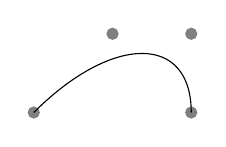
\begin{tikzpicture}
    \filldraw [gray] (0,0) circle [radius=2pt] (1,1) circle
    [radius=2pt] (2,1) circle [radius=2pt] (2,0) circle [radius=2pt];
    \draw (0,0) .. controls (1,1) and (2,1) .. (2,0);
  \end{tikzpicture}
  \begin{tikzpicture}
    \draw (-1.5,0) -- (1.5,0); \draw (0,-1.5) -- (0,1.5); \draw (-1,0)
    .. controls (-1,0.555) and (-0.555,1) .. (0,1) .. controls
    (0.555,1) and (1,0.555) .. (1,0);
  \end{tikzpicture}
  \begin{tikzpicture}
    \draw (-1.5,0) -- (1.5,0); \draw (0,-1.5) -- (0,1.5); \draw (-1,0)
    .. controls (-1,0.577) and (-0.577,1) .. (0,1) .. controls
    (0.577,1) and (1,0.577) .. (1,0);
  \end{tikzpicture}
  \begin{tikzpicture}
    \draw (-1.5,0) -- (1.5,0); \draw (0,-1.5) -- (0,1.5); \draw (-1,0)
    .. controls (-0.707,0.707) .. (0,1) .. controls (0.707,0.707)
    .. (1,0);
  \end{tikzpicture}
\end{frame}

\begin{frame}[fragile]
  \frametitle{圆}

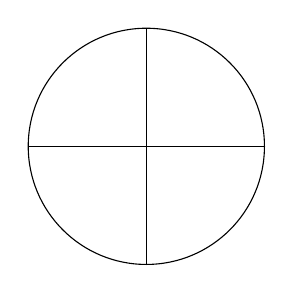
\begin{tikzpicture}
  \draw (-1.5,0) -- (1.5,0); \draw (0,-1.5) -- (0,1.5); \draw (0,0)
  circle [radius=1.5];
\end{tikzpicture}
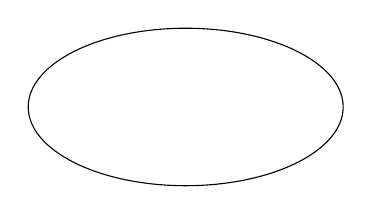
\begin{tikzpicture}
  \draw (0,0) ellipse [x radius=2, y radius=1];
\end{tikzpicture}
\end{frame}

\begin{frame}[fragile] \frametitle{矩形}
  \begin{center}
    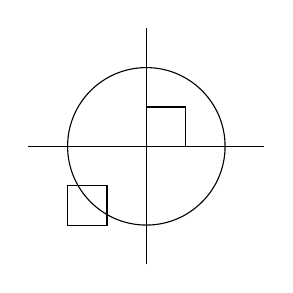
\begin{tikzpicture}
      \draw (-1.5,0) -- (1.5,0); \draw (0,-1.5) -- (0,1.5); \draw
      (0,0) circle [radius=1cm]; \draw (0,0) rectangle (0.5,0.5);
      \draw (-0.5,-0.5) rectangle (-1,-1);
    \end{tikzpicture}
  \end{center}
\end{frame}

\begin{frame}[fragile]\frametitle{网格}
  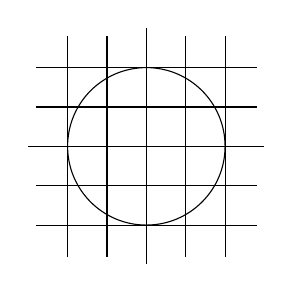
\begin{tikzpicture}
    \draw (-1.5,0) -- (1.5,0); \draw (0,-1.5) -- (0,1.5); \draw (0,0)
    circle [radius=1cm]; \draw[step=.5cm] (-1.4,-1.4) grid (1.4,1.4);
  \end{tikzpicture}
  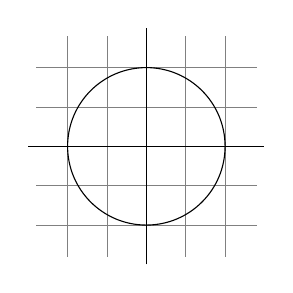
\begin{tikzpicture}
    \draw[step=.5cm,gray,very thin] (-1.4,-1.4) grid (1.4,1.4); \draw
    (-1.5,0) -- (1.5,0); \draw (0,-1.5) -- (0,1.5); \draw (0,0) circle
    [radius=1cm];
  \end{tikzpicture}
\end{frame}

\begin{frame}[fragile]\frametitle{自定义样式}
  \tikzset{help lines/.style=very thin} \tikzset{Karl’s
    grid/.style={help lines,color=blue!50}}

\begin{tikzpicture}
[Karl’s grid/.style ={help lines,color=#1!50},Karl’s grid/.default=blue]
\draw[Karl’s grid,step=1] (0,0) grid (5,5); \draw[Karl’s
grid=red,step=1cm,xshift=0.5cm] (5.5,0.5) grid (10.5,4.5);
\end{tikzpicture}
\begin{tikzpicture} [Karl’s grid/.style ={help lines,color=#1!50},
  Karl’s grid/.default=blue]
  \draw[Karl’s grid] (0,0) grid (1.5,2); \draw[Karl’s grid=red]
  (2,0) grid (3.5,2);
\end{tikzpicture}
\end{frame}

\begin{frame}[fragile]\frametitle{弧段}
  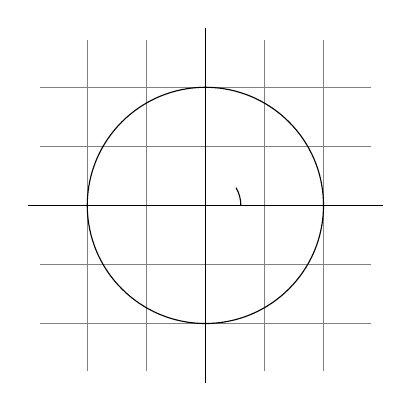
\begin{tikzpicture}[scale=1.5]
    \draw[step=.5cm,gray,very thin] (-1.4,-1.4) grid (1.4,1.4); \draw
    (-1.5,0) -- (1.5,0); \draw (0,-1.5) -- (0,1.5); \draw (0,0) circle
    [radius=1cm]; \draw (3mm,0mm) arc [start angle=0, end angle=30,
    radius=3mm];
  \end{tikzpicture}
  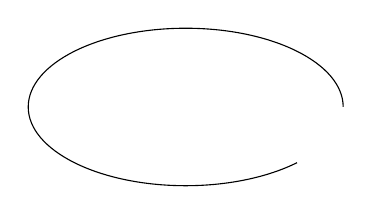
\begin{tikzpicture}
    \draw (0,0) arc [start angle=0, end angle=315, x radius=2, y
    radius=1];
  \end{tikzpicture}
\end{frame}

\begin{frame}[fragile]\frametitle{切割图形}
  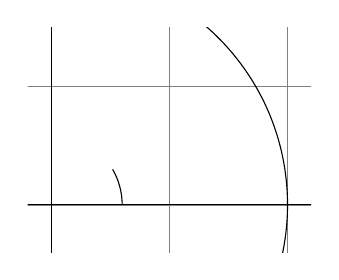
\begin{tikzpicture}[scale=3]
    \clip (-0.1,-0.2) rectangle (1.1,0.75); \draw[step=.5cm,gray,very
    thin] (-1.4,-1.4) grid (1.4,1.4); \draw (-1.5,0) -- (1.5,0); \draw
    (0,-1.5) -- (0,1.5); \draw (0,0) circle [radius=1cm]; \draw
    (3mm,0mm) arc [start angle=0, end angle=30, radius=3mm];
  \end{tikzpicture}
  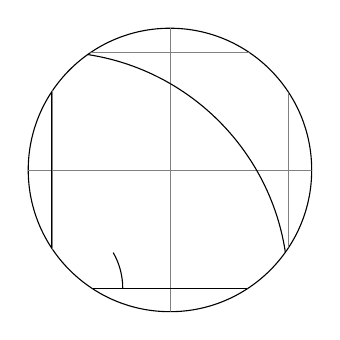
\begin{tikzpicture}[scale=3]
    \clip[draw] (0.5,0.5) circle (.6cm); \draw[step=.5cm,gray,very
    thin] (-1.4,-1.4) grid (1.4,1.4); \draw (-1.5,0) -- (1.5,0); \draw
    (0,-1.5) -- (0,1.5); \draw (0,0) circle [radius=1cm]; \draw
    (3mm,0mm) arc [start angle=0, end angle=30, radius=3mm];
  \end{tikzpicture}
\end{frame}

\begin{frame}[fragile]\frametitle{抛物线}
  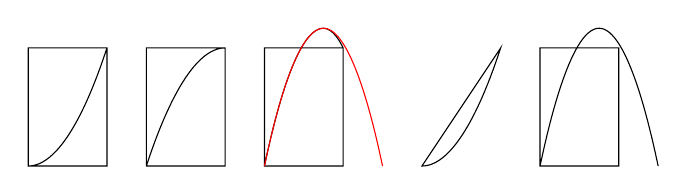
\begin{tikzpicture}
    \draw (0,0) rectangle (1,1.5) (0,0) parabola (1,1.5);
    \draw[xshift=1.5cm] (0,0) rectangle (1,1.5) (0,0) parabola[bend at
    end] (1,1.5); \draw[xshift=3cm] (0,0) rectangle (1,1.5) (0,0)
    parabola bend (.75,1.75) (1,1.5); \draw[xshift=3cm,color=red]
    (0,0) parabola bend (.75,1.75) (1.5,0); \draw[xshift=5cm] (1,1.5)
    --(0,0) parabola cycle; \draw[xshift=6.5cm] (0,0) rectangle
    (1,1.5) (0,0) parabola bend (.75,1.75) (1.5,0);
  \end{tikzpicture}
\end{frame}

\begin{frame}[fragile]\frametitle{正弦和余弦}
  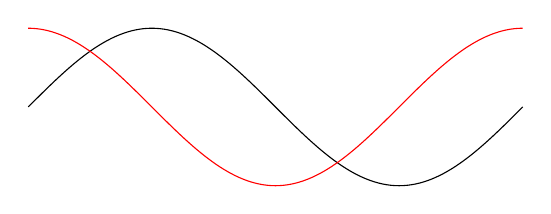
\begin{tikzpicture}[xscale=1.57]
    \draw (0,0) sin (1,1) cos (2,0) sin (3,-1) cos (4,0);
    \draw[color=red] (0,1) cos (1,0) sin (2,-1) cos (3,0) sin (4,1);
  \end{tikzpicture}
\end{frame}

\begin{frame}[fragile]\frametitle{填充}
  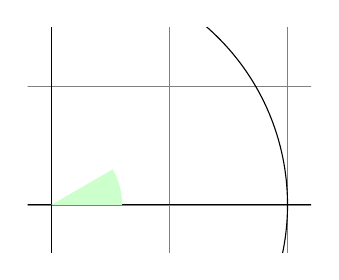
\begin{tikzpicture}[scale=3]
    \clip (-0.1,-0.2) rectangle (1.1,0.75); \draw[step=.5cm,gray,very
    thin] (-1.4,-1.4) grid (1.4,1.4); \draw (-1.5,0) -- (1.5,0); \draw
    (0,-1.5) -- (0,1.5); \draw (0,0) circle [radius=1cm];
    \fill[green!20!white] (0,0) -- (3mm,0mm) arc [start angle=0, end
    angle=30, radius=3mm] -- (0,0);
  \end{tikzpicture}
  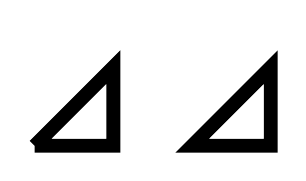
\begin{tikzpicture}[line width=5pt]
    \draw (0,0) -- (1,0) -- (1,1) -- (0,0); \draw (2,0) -- (3,0) --
    (3,1) -- cycle; \useasboundingbox
    (0,1.5); % make bounding box higher
  \end{tikzpicture}
  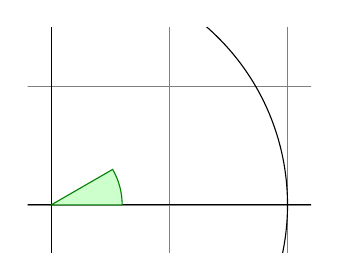
\begin{tikzpicture}[scale=3]
    \clip (-0.1,-0.2) rectangle (1.1,0.75); \draw[step=.5cm,gray,very
    thin] (-1.4,-1.4) grid (1.4,1.4); \draw (-1.5,0) -- (1.5,0); \draw
    (0,-1.5) -- (0,1.5); \draw (0,0) circle [radius=1cm];
    \filldraw[fill=green!20!white, draw=green!50!black] (0,0) --
    (3mm,0mm) arc [start angle=0, end angle=30, radius=3mm] -- cycle;
  \end{tikzpicture}
\end{frame}

\begin{frame}[fragile]\frametitle{阴影渐变色}
  
\begin{tikzpicture}
    \shade (0,0) rectangle (2,1) (3,0.5) circle (.5cm);
  \end{tikzpicture}


\begin{tikzpicture}[rounded corners,ultra thick]
  \shade[top color=yellow,bottom color=black] (0,0) rectangle +(2,1);
  \shade[left color=yellow,right color=black] (3,0) rectangle +(2,1);
  \shadedraw[inner color=yellow,outer color=black,draw=yellow] (6,0)
  rectangle +(2,1); \shade[ball color=green] (9,.5) circle (.5cm);
\end{tikzpicture}

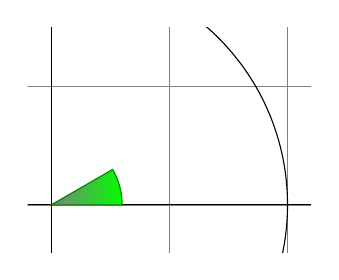
\begin{tikzpicture}[scale=3]
  \clip (-0.1,-0.2) rectangle (1.1,0.75); \draw[step=.5cm,gray,very
  thin] (-1.4,-1.4) grid (1.4,1.4); \draw (-1.5,0) -- (1.5,0); \draw
  (0,-1.5) -- (0,1.5); \draw (0,0) circle [radius=1cm];
  \shadedraw[left color=gray,right color=green, draw=green!50!black]
  (0,0) -- (3mm,0mm) arc [start angle=0, end angle=30, radius=3mm] --
  cycle;
\end{tikzpicture}
\end{frame}

\begin{frame}[fragile]\frametitle{特定坐标}
  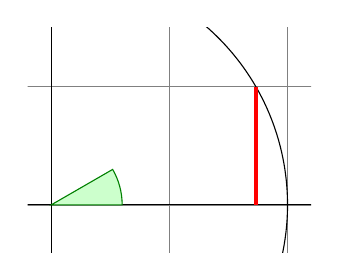
\begin{tikzpicture}[scale=3]
    \clip (-0.1,-0.2) rectangle (1.1,0.75); \draw[step=.5cm,gray,very
    thin] (-1.4,-1.4) grid (1.4,1.4); \draw (-1.5,0) -- (1.5,0); \draw
    (0,-1.5) -- (0,1.5); \draw (0,0) circle [radius=1cm];
    \filldraw[fill=green!20,draw=green!50!black] (0,0) -- (3mm,0mm)
    arc [start angle=0, end angle=30, radius=3mm] -- cycle;
    \draw[red,very thick] (30:1cm) -- +(0,-0.5);
  \end{tikzpicture}
  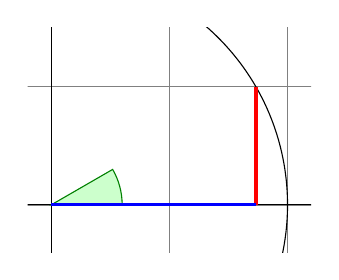
\begin{tikzpicture}[scale=3]
    \clip (-0.1,-0.2) rectangle (1.1,0.75); \draw[step=.5cm,gray,very
    thin] (-1.4,-1.4) grid (1.4,1.4); \draw (-1.5,0) -- (1.5,0); \draw
    (0,-1.5) -- (0,1.5); \draw (0,0) circle [radius=1cm];
    \filldraw[fill=green!20,draw=green!50!black] (0,0) -- (3mm,0mm)
    arc [start angle=0, end angle=30, radius=3mm] -- cycle;
    \draw[red,very thick] (30:1cm) -- +(0,-0.5); \draw[blue,very
    thick] (30:1cm) ++(0,-0.5) -- (0,0);
  \end{tikzpicture}
\end{frame}

\begin{frame}[fragile]\frametitle{相交路径}
  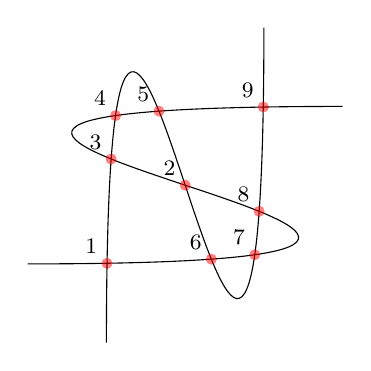
\begin{tikzpicture}
    \clip (-2,-2) rectangle (2,2); \draw [name path=curve 1] (-2,-1)
    .. controls (8,-1) and (-8,1) .. (2,1); \draw [name path=curve 2]
    (-1,-2) .. controls (-1,8) and (1,-8) .. (1,2); \fill [name
    intersections={of=curve 1 and curve 2, name=i, total=\t}] [red,
    opacity=0.5, every node/.style={above left, black, opacity=1}]
    \foreach \s in {1,...,\t}{(i-\s) circle (2pt) node
      {\footnotesize\s}};
  \end{tikzpicture}
  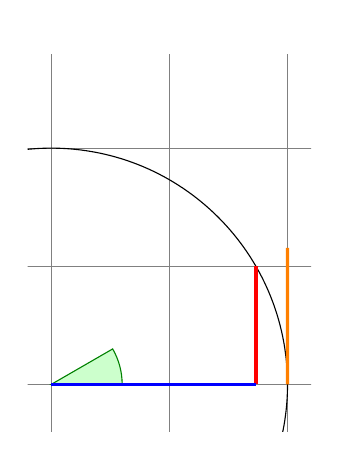
\begin{tikzpicture}[scale=3]
    \clip (-0.1,-0.2) rectangle (1.1,1.51); \draw[step=.5cm,gray,very
    thin] (-1.4,-1.4) grid (1.4,1.4); \draw (0,0) circle [radius=1cm];
    \filldraw[fill=green!20,draw=green!50!black] (0,0) -- (3mm,0mm)
    arc [start angle=0, end angle=30, radius=3mm] -- cycle;
    \draw[red,very thick] (30:1cm) -- +(0,-0.5); \draw[blue,very
    thick] (30:1cm) ++(0,-0.5) -- (0,0); \path [name path=upward line]
    (1,0) -- (1,1); \path [name path=sloped line] (0,0) -- (30:1.5cm);
    \draw [name intersections={of=upward line and sloped line, by=x}]
    [very thick,orange] (1,0) -- (x);
  \end{tikzpicture}
\end{frame}

\begin{frame}[fragile]\frametitle{箭头}
   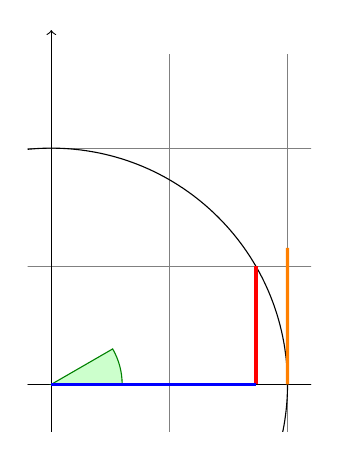
\begin{tikzpicture}[scale=3]
     \clip (-0.1,-0.2) rectangle (1.1,1.51); \draw[step=.5cm,gray,very
     thin] (-1.4,-1.4) grid (1.4,1.4); \draw[->] (-1.5,0) -- (1.5,0);
     \draw[->] (0,-1.5) -- (0,1.5); \draw (0,0) circle [radius=1cm];
     \filldraw[fill=green!20,draw=green!50!black] (0,0) -- (3mm,0mm)
     arc [start angle=0, end angle=30, radius=3mm] -- cycle;
     \draw[red,very thick] (30:1cm) -- +(0,-0.5); \draw[blue,very
     thick] (30:1cm) ++(0,-0.5) -- (0,0);

     \path [name path=upward line] (1,0) -- (1,1); \path [name
      path=sloped line] (0,0) -- (30:1.5cm); \draw [name
      intersections={of=upward line and sloped line, by=x}] [very
      thick,orange] (1,0) -- (x);
   \end{tikzpicture}
   \begin{tikzpicture}[scale=3]
      \draw [<->] (0,0) arc [start angle=180, end angle=30,
      radius=10pt]; \draw [<->] (1,0) -- (1.5cm,10pt) -- (2cm,0pt) --
      (2.5cm,10pt);
   \end{tikzpicture}
\end{frame}

 \begin{frame}[fragile]\frametitle{范围}
   \begin{tikzpicture}[ultra thick]
     \draw (0,0) -- (0,1);
     \begin{scope}[thin]
       \draw (1,0) -- (1,1); \draw (2,0) -- (2,1);
     \end{scope}
     \draw (3,0) -- (3,1);
   \end{tikzpicture}
 \end{frame}

\begin{frame}[fragile]\frametitle{位置转换}
  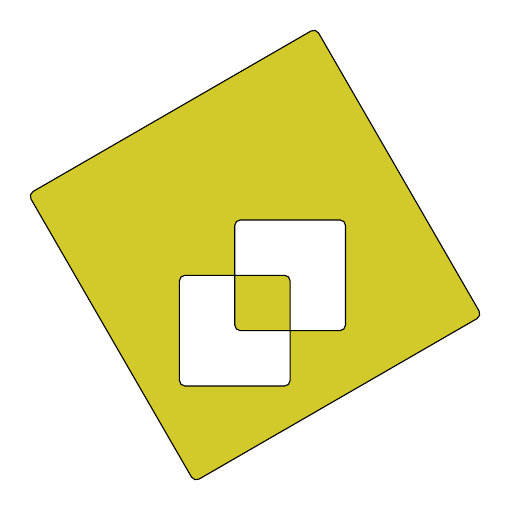
\begin{tikzpicture}[even odd rule,rounded
    corners=2pt,x=10pt,y=10pt,scale=4]
    \filldraw[fill=yellow!80!black] (0,0) rectangle (1,1)
    [xshift=5pt,yshift=5pt] (0,0) rectangle (1,1) [rotate=30] (-1,-1)
    rectangle (2,2);
  \end{tikzpicture}
\end{frame}

\begin{frame}[fragile]\frametitle{循环}
  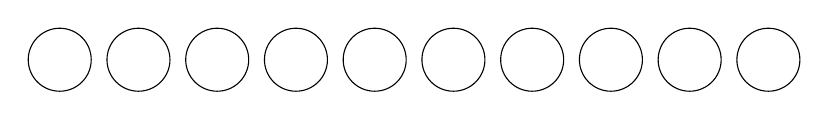
\begin{tikzpicture}
    \foreach \x in {1,...,10} \draw (\x,0) circle (0.4cm);
  \end{tikzpicture}
  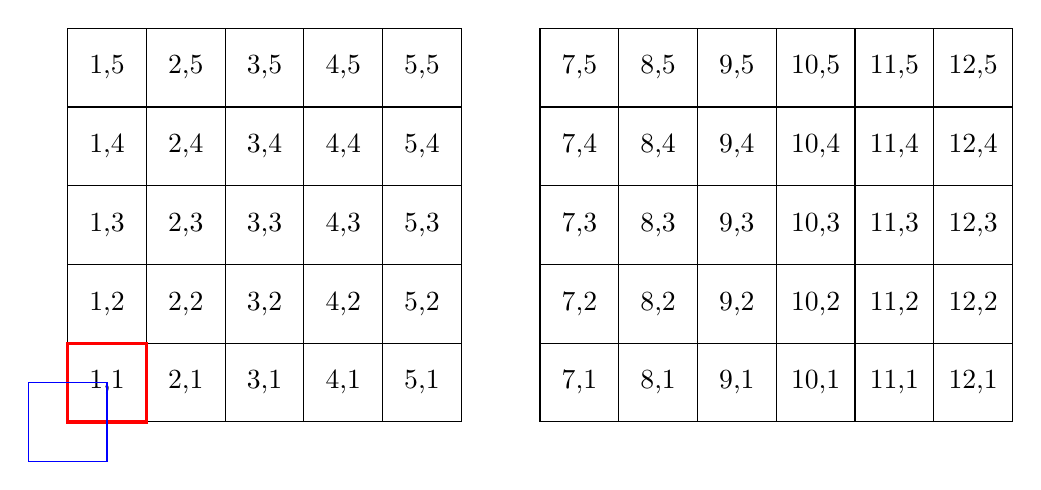
\begin{tikzpicture}
    \foreach \x in {1,2,...,5,7,8,...,12} 
    \foreach \y in {1,...,5} {
      \draw (\x,\y) +(-.5,-.5) rectangle ++(.5,.5); 
      \draw (\x,\y) node{\x,\y}; }
    \draw[color=red,very thick] (1,1) +(-0.5,-0.5) rectangle ++(0.5,0.5);
    \draw[color=blue] (0,0) rectangle (1,1);
  \end{tikzpicture}
\end{frame}

\begin{frame}[fragile]\frametitle{添加文字(1)}
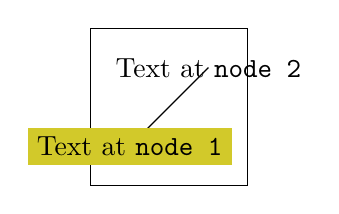
\begin{tikzpicture}
\draw (0,0) rectangle (2,2);
\draw (0.5,0.5) node [fill=yellow!80!black]
{Text at \verb!node 1!}
-- (1.5,1.5) node {Text at \verb!node 2!};
\end{tikzpicture} 
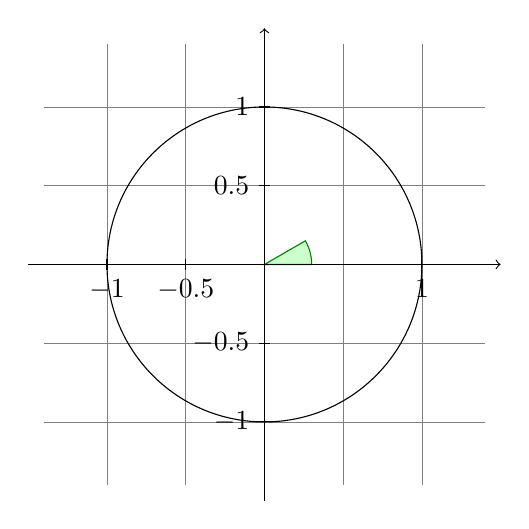
\begin{tikzpicture}[scale=2]
%\clip (-0.6,-0.2) rectangle (0.6,1.51);
\draw[step=.5cm,help lines] (-1.4,-1.4) grid (1.4,1.4);
\filldraw[fill=green!20,draw=green!50!black] (0,0) -- (3mm,0mm)
arc [start angle=0, end angle=30, radius=3mm] -- cycle;
\draw[->] (-1.5,0) -- (1.5,0); \draw[->] (0,-1.5) -- (0,1.5);
\draw (0,0) circle [radius=1cm];
\foreach \x in {-1,-0.5,1}
\draw (\x cm,1pt) -- (\x cm,-1pt) node[anchor=north] {$\x$};
\foreach \y in {-1,-0.5,0.5,1}
\draw (1pt,\y cm) -- (-1pt,\y cm) node[anchor=east] {$\y$};
\end{tikzpicture} 
\end{frame}

\begin{frame}[fragile]\frametitle{添加文字(2)}
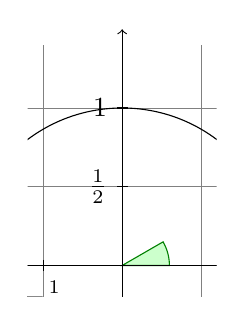
\begin{tikzpicture}[scale=2]
\clip (-0.6,-0.2) rectangle (0.6,1.51);
\draw[step=.5cm,help lines] (-1.4,-1.4) grid (1.4,1.4);
\filldraw[fill=green!20,draw=green!50!black] (0,0) -- (3mm,0mm)
arc [start angle=0, end angle=30, radius=3mm] -- cycle;
\draw[->] (-1.5,0) -- (1.5,0); \draw[->] (0,-1.5) -- (0,1.5);
\draw (0,0) circle [radius=1cm];
\foreach \x/\xtext in {-1, -0.5/-\frac{1}{2}, 1}
\draw (\x cm,1pt) -- (\x cm,-1pt) node[anchor=north] {$\xtext$};
\foreach \y/\ytext in {-1, -0.5/-\frac{1}{2}, 0.5/\frac{1}{2}, 1}
\draw (1pt,\y cm) -- (-1pt,\y cm) node[anchor=east] {$\ytext$};
\end{tikzpicture}
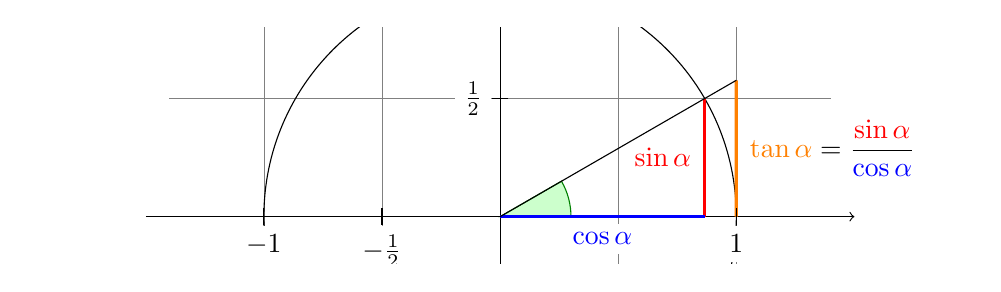
\begin{tikzpicture}[scale=3]
\clip (-2,-0.2) rectangle (2,0.8);
\draw[step=.5cm,gray,very thin] (-1.4,-1.4) grid (1.4,1.4);
\filldraw[fill=green!20,draw=green!50!black] (0,0) -- (3mm,0mm)
arc [start angle=0, end angle=30, radius=3mm] -- cycle;
\draw[->] (-1.5,0) -- (1.5,0) coordinate (x axis);
\draw[->] (0,-1.5) -- (0,1.5) coordinate (y axis);
\draw (0,0) circle [radius=1cm];
\draw[very thick,red]
(30:1cm) -- node[left=1pt,fill=white] {$\sin \alpha$} (30:1cm |- x axis);
\draw[very thick,blue]
(30:1cm |- x axis) -- node[below=2pt,fill=white] {$\cos \alpha$} (0,0);
\path [name path=upward line] (1,0) -- (1,1);
\path [name path=sloped line] (0,0) -- (30:1.5cm);
\draw [name intersections={of=upward line and sloped line, by=t}]
[very thick,orange] (1,0) -- node [right=1pt,fill=white]
{$\displaystyle \tan \alpha \color{black}=
\frac{{\color{red}\sin \alpha}}{\color{blue}\cos \alpha}$} (t);
\draw (0,0) -- (t);
\foreach \x/\xtext in {-1, -0.5/-\frac{1}{2}, 1}
\draw (\x cm,1pt) -- (\x cm,-1pt) node[anchor=north,fill=white] {$\xtext$};
\foreach \y/\ytext in {-1, -0.5/-\frac{1}{2}, 0.5/\frac{1}{2}, 1}
\draw (1pt,\y cm) -- (-1pt,\y cm) node[anchor=east,fill=white] {$\ytext$};
\end{tikzpicture}  
\end{frame}

\begin{frame}[fragile]\frametitle{完整结果}
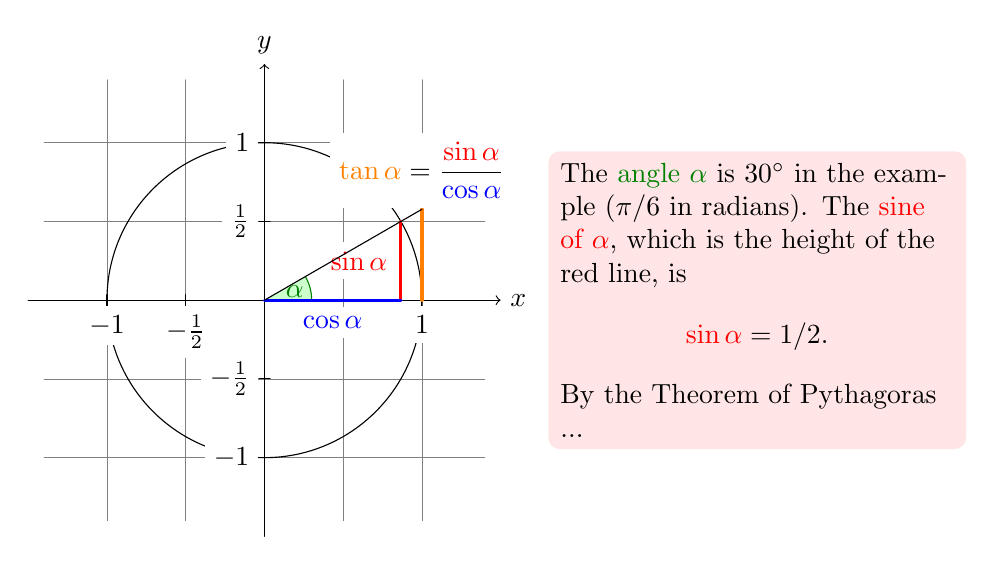
\begin{tikzpicture}
[scale=2,line cap=round,
% Styles
axes/.style=,
important line/.style={very thick},
information text/.style={rounded corners,fill=red!10,inner sep=1ex}]
% Colors
\colorlet{anglecolor}{green!50!black}
\colorlet{sincolor}{red}
\colorlet{tancolor}{orange!80!black}
\colorlet{coscolor}{blue}
% The graphic
\draw[help lines,step=0.5cm] (-1.4,-1.4) grid (1.4,1.4);
\draw (0,0) circle [radius=1cm];
\begin{scope}[axes]
\draw[->] (-1.5,0) -- (1.5,0) node[right] {$x$} coordinate(x axis);
\draw[->] (0,-1.5) -- (0,1.5) node[above] {$y$} coordinate(y axis);
\foreach \x/\xtext in {-1, -.5/-\frac{1}{2}, 1}
\draw[xshift=\x cm] (0pt,1pt) -- (0pt,-1pt) node[below,fill=white] {$\xtext$};
\foreach \y/\ytext in {-1, -.5/-\frac{1}{2}, .5/\frac{1}{2}, 1}
\draw[yshift=\y cm] (1pt,0pt) -- (-1pt,0pt) node[left,fill=white] {$\ytext$};
\end{scope}
\filldraw[fill=green!20,draw=anglecolor] (0,0) -- (3mm,0pt)
arc [start angle=0, end angle=30, radius=3mm];
\draw (15:2mm) node[anglecolor] {$\alpha$};
\draw[important line,sincolor]
(30:1cm) -- node[left=1pt,fill=white] {$\sin \alpha$} (30:1cm |- x axis);
\draw[important line,coscolor]
(30:1cm |- x axis) -- node[below=2pt,fill=white] {$\cos \alpha$} (0,0);
\path [name path=upward line] (1,0) -- (1,1);
\path [name path=sloped line] (0,0) -- (30:1.5cm);
\draw [name intersections={of=upward line and sloped line, by=t}]
[very thick,orange] (1,0) -- (t)
node [anchor=south,fill=white]
{$\displaystyle \tan \alpha \color{black}=
\frac{{\color{red}\sin \alpha}}{\color{blue}\cos \alpha}$};
\draw (0,0) -- (t);
\draw[xshift=1.8cm]
node[right,text width=5cm,information text]
{
The {\color{anglecolor} angle $\alpha$} is $30^\circ$ in the
example ($\pi/6$ in radians). The {\color{sincolor}sine of
$\alpha$}, which is the height of the red line, is
\[
{\color{sincolor} \sin \alpha} = 1/2.
\]
By the Theorem of Pythagoras ...
};
\end{tikzpicture}  
\end{frame}
\end{document}
